\chapter{Example of an illustrative application}

 To contextualize the practical rendering, it is currently possible to implement static digitization using any \textit{openstreetmap} file and specifying some parameters arbitrarily for the demography of the territory. Dynamic digitalization is very simplistic and carried out completely randomly. The infectious implementation allows automatic management of infectious transitions. The concrete rendering therefore corresponds to the digitization of the Belval university campus, in Esch-sur-Alzette, over a predetermined number of days, and with an infectious initialization to be arbitrarily defined. The basis of digitalization really needs to be consolidated, whether static or dynamic. This is just the beginning of the work. My last experiments were to play with the parameters of an infection, including the threshold of contamination, and to empirically observe the infectious evolutions of the population on a graph.\\

\pagebreak

\begin{figure}[h]
  \centering
  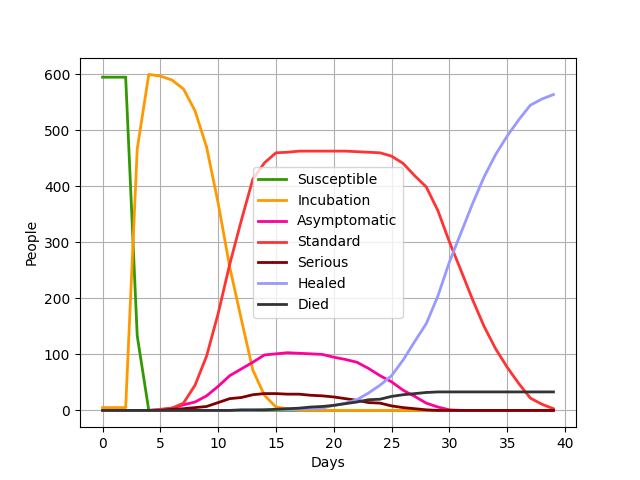
\includegraphics[width=\linewidth]{Media/ExperimentationBelval.png}
  \caption{\centering {\small An illustrative example of infectious curves with the current implementation.}}
  \label{fig:experimentationbelval}
\end{figure}

Quickly, we can get an overview of the design on the digitalization of an epidemic with the graph above. Without going into details, this test was carried out with cartographic data from the Belval campus in Esch-sur-Alzette. Six hundred individuals were implemented, over a period of forty days. Every day their dynamics are totally random and cover the entire network. So we can see it as a totally related graph where all individuals necessarily intersect. There are no outside considerations here. The test was carried out with five individuals in the incubation phase from day one.\\

There is very unrealistic contamination. Even if all individuals rub shoulders daily without exception, it seems irrational to see the entire population become infected so quickly ; Hence the interest of implementing a form of elasticity in the contamination threshold. Indeed, the dynamic profile is almost identical for all individuals : we therefore find contamination scores too similar to observe a dispersion of infections. After, we can find a fairly well-known graph with the news. There is an exponential increase in sick cases as well as a ``leveling off''. In reality, asymptomatic patients are not identified and the network of proximity between individuals is less connected. We can of course review the proportions between infectious severities ; no attempt has been made to replicate actual Covid-19 data. In addition, no care has been implemented, hence the fatality of individuals in serious condition and the increase in the number of individuals who die. Vaccinations have also not been implemented here.\\

The practical realization and everything that surrounds its production can be treated during a defense. We can then address the structural management of memory management, decisions for static digitalization or problem solving in the dynamics of society. It will be much more explicit and stimulating than evoking all the theoretical reflections.